% !TeX program = xelatex 

\PassOptionsToPackage{prologue, dvipsnames}{xcolor}
\documentclass[AutoFakeBold,AutoFakeSlant]{article}
\usepackage{listings}

% 支持中文的设置
\usepackage{xeCJK}
\usepackage{fontspec}
\setCJKmainfont[ItalicFont=思源宋体,BoldFont=SourceHanSerifSC-Bold]{Source Han Serif SC}
\newcommand{\KaiTi}{\CJKfontspec{楷体}}%用命令\fzkaiti调用方正楷体简体

% other packages
\usepackage{subfigure}
\usepackage{latexsym,amsmath,xcolor,multicol,booktabs,calligra}
\usepackage{graphicx,pstricks,listings,stackengine}

\usepackage{geometry}
\geometry{left=2cm,right=2cm,top=2cm,bottom=2cm}

\lstnewenvironment{cppcode}[1][]%
{
	\lstset{
		tabsize=4,
		language={C++},
		escapeinside=``,
		breaklines=true,
		frame=shadowbox, %把代码用带有阴影的框圈起来
		breakatwhitespace=true, % 在空格处断行
		basicstyle=\ttfamily,
		keywordstyle=\color{blue}\ttfamily,
		stringstyle=\color{red}\ttfamily,
		commentstyle=\color{green}\ttfamily,
		morecomment=[l][\color{magenta}]{\#},
		literate={\ \ }{{\ \ \ \ }}4,
		#1
	}
}%
{}



\lstnewenvironment{cmakecode}[1][]%
{
	\lstset{
		tabsize=4,
		language={CMake},
		escapeinside=``,
		breaklines=true,
		frame=shadowbox,
		breakatwhitespace=true,
		basicstyle=\ttfamily,
		keywordstyle=\color{blue}\ttfamily,
		stringstyle=\color{red}\ttfamily,
		commentstyle=\color{green}\ttfamily,
		morecomment=[l][\color{magenta}]{\#},
		literate={\ \ }{{\ \ \ \ }}4,
			#1
	}
}%
{}
	
\begin{document}
	
	\begin{center}
		\Huge 
		Boost 安装 (Windows x86)
	\end{center}
	
	\leftline
	\bigskip
	\begin{flushleft}
		\begin{huge}
			一、 安装过程
		\end{huge}
		
		\large 
		\linespread{1.2} \selectfont
		\begin{enumerate}
			\item 下载boost安装包,如(boost\_1\_83\_0.7z),解压到本地目录,如D:/boost-1.83.0
			\item 运行D:/boost-1.83.0/bootstrap.bat,会在同目录下生成b2.exe
			\item .\b2.exe toolset=msvc-14.3 install --prefix=D:/boost-1.83.0 link=static
		\end{enumerate}
		
		\bigskip
		
		上面命令生成的库为静态库,包括release、debug版本,64位、32位版本,支持多线程,使用的编译器为msvc14.3(对应vs2022),足以满足需要了。安装位置为e:/dev/boost。若不指定--prefix=D:/boost-1.83.0,则安装地址默认为c:/boost。
		
		\bigskip
		
		\textbf{一般以静态库方式使用boost。}
		
		
		\vspace{3cm}
		
		\begin{huge}
			二、 安装测试
		\end{huge}
		
		\bigskip
		\large
		1. CMakeList测试环境构建
		\begin{cmakecode}
cmake_minimum_required( VERSION 3.5.1)
project(BOOST)

set(CMAKE_PREFIX_PATH D:/boost-1.83.0/boost-1.83.0)

find_package(Boost COMPONENTS thread REQUIRED)
INCLUDE_DIRECTORIES( ${Boost_INCLUDE_DIR} )
LINK_DIRECTORIES( ${Boost_LIBRARY_DIRS} )
set( Boost_USE_STATIC_LIBS        OFF )
set( Boost_USE_MULTITHREADED      ON )
set( Boost_USE_STATIC_RUNTIME     OFF )
set( BOOST_ALL_DYN_LINK           ON )

add_executable( ${PROJECT_NAME} HelloThreader.cpp )
target_link_libraries( ${PROJECT_NAME} ${Boost_LIBRARIES})
		\end{cmakecode}
		
	\end{flushleft}
	
	\clearpage	
	
	\begin{flushleft}
		\large
		2. HelloThreader.cpp测试线程模块是否正确引入
		\begin{cppcode}
#include <iostream>
#include <boost/thread/thread.hpp>

void threadFunction() {
	for (int i = 0; i < 5; ++i) {
		std::cout << "Thread running: " << i << std::endl;
		boost::this_thread::sleep(boost::posix_time::milliseconds(1000));  // 休眠1秒
	}
}

int main() {
	// 启动一个新线程
	boost::thread myThread(&threadFunction);
	
	// 主线程继续执行其他任务
	for (int i = 0; i < 3; ++i) {
		std::cout << "Main thread running: " << i << std::endl;
		boost::this_thread::sleep(boost::posix_time::milliseconds(500));  // 休眠0.5秒
	}
	
	// 等待子线程结束
	myThread.join();
	
	return 0;
}
		\end{cppcode}
	\end{flushleft}
	
	\begin{flushleft}
		\begin{figure*}[htbp]
			\centering
			\subfigure[正常编译运行测试结果]{
				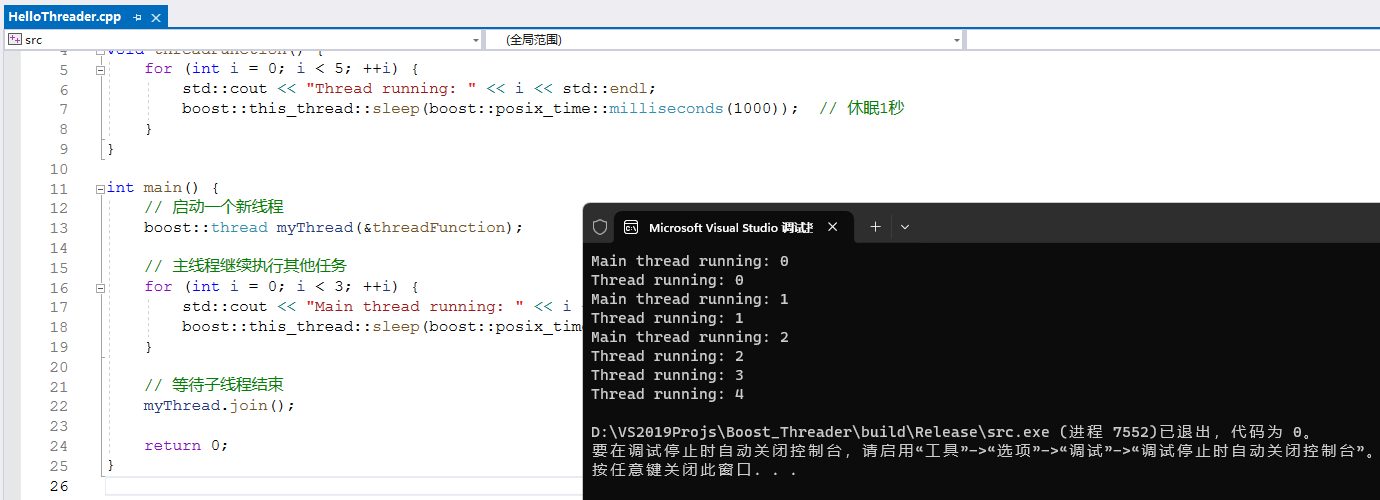
\includegraphics[width=\linewidth]{BoostThreaderResult}
			} 
		\end{figure*}
	\end{flushleft}
\end{document}
